% Fonte da figura imagens/grafo-coleta.pdf, usada no exemplo de TCC.
% Para regerar o PDF (a partir da pasta imagens/):
%   pdflatex grafo-coleta.tex
\documentclass[tikz,border=4pt]{standalone}
\usepackage[T1]{fontenc}
\usepackage{helvet}
\renewcommand{\familydefault}{\sfdefault}
\usetikzlibrary{positioning}

\begin{document}
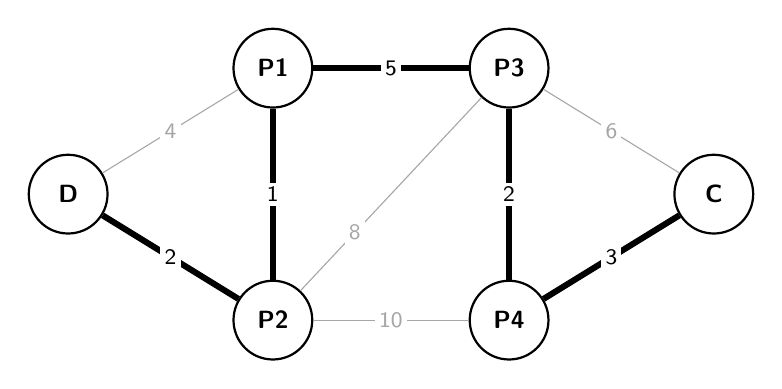
\begin{tikzpicture}[
    ponto/.style={circle, draw, thick, minimum size=10mm, font=\small\bfseries},
    via/.style={draw, gray!70},
    rota/.style={draw, line width=2.2pt},
    peso/.style={font=\footnotesize, fill=white, inner sep=1.5pt}
  ]
  \node[ponto] (D)  at (0,0)     {D};
  \node[ponto] (P2) at (2.6,-1.6) {P2};
  \node[ponto] (P1) at (2.6,1.6)  {P1};
  \node[ponto] (P3) at (5.6,1.6)  {P3};
  \node[ponto] (P4) at (5.6,-1.6) {P4};
  \node[ponto] (C)  at (8.2,0)    {C};

  % vias que não fazem parte da rota mínima
  \draw[via] (D)  -- node[peso] {4}  (P1);
  \draw[via] (P2) -- node[peso, pos=0.3] {8}  (P3);
  \draw[via] (P2) -- node[peso] {10} (P4);
  \draw[via] (P3) -- node[peso] {6}  (C);

  % rota mínima de D até C: D-P2-P1-P3-P4-C (13 km)
  \draw[rota] (D)  -- node[peso] {2} (P2);
  \draw[rota] (P2) -- node[peso] {1} (P1);
  \draw[rota] (P1) -- node[peso] {5} (P3);
  \draw[rota] (P3) -- node[peso] {2} (P4);
  \draw[rota] (P4) -- node[peso] {3} (C);
\end{tikzpicture}
\end{document}
